%%%%%%%%%%%%%%%%%%%%%%%%%%%%%%%%%%%%%%%%%%%%%%%%%%%%%%%%%%%%
% 1.10 NONCOMMUTATIVE ALGEBRA
% The Composition of Advanced Mathematics
%%%%%%%%%%%%%%%%%%%%%%%%%%%%%%%%%%%%%%%%%%%%%%%%%%%%%%%%%%%%

\section{Noncommutative Algebra}
\label{sec:noncommutative-algebra}

\prerequisite{
Abstract algebra from \cref{sec:abstract-algebra}, group theory from
\cref{sec:group-theory}, ring theory from \cref{sec:ring-theory}, and
module theory from \cref{sec:module-theory}.
}

\learningobjectives{
By the end of this section, the reader should be able to:
\begin{itemize}
    \item explain what makes a ring noncommutative;
    \item recognize important examples of noncommutative rings;
    \item distinguish left ideals, right ideals, and two-sided ideals;
    \item distinguish left modules from right modules;
    \item compute commutators and interpret central elements;
    \item determine the center of basic noncommutative rings;
    \item work with matrix rings and endomorphism rings;
    \item define opposite rings and understand their purpose;
    \item distinguish units, zero divisors, and nilpotent elements in noncommutative settings;
    \item work with division rings and understand the role of quaternions;
    \item define simple rings and recognize matrix rings as fundamental examples;
    \item understand minimal left ideals and simple modules;
    \item explain the Jacobson radical at an introductory level;
    \item recognize chain conditions in noncommutative rings;
    \item understand the basic structure of semisimple rings;
    \item state the Artin--Wedderburn theorem and interpret its meaning;
    \item recognize group algebras and free associative algebras;
    \item explain how noncommutative algebra connects ring theory, representation theory, and operator theory.
\end{itemize}
}

%%%%%%%%%%%%%%%%%%%%%%%%%%%%%%%%%%%%%%%%%%%%%%%%%%%%%%%%%%%%
\subsection{When Multiplication Does Not Commute}
\label{subsec:noncommutative-multiplication}
%%%%%%%%%%%%%%%%%%%%%%%%%%%%%%%%%%%%%%%%%%%%%%%%%%%%%%%%%%%%

In a commutative ring,

\[ ab=ba \]

for every pair of elements.

Noncommutative algebra studies algebraic systems in which this equality is
not assumed.

Thus there may exist \(a,b\in R\) such that

\[ ab\neq ba. \]

\begin{definitionbox}{Noncommutative Ring}
A ring \(R\) is called \emph{noncommutative} if there exist elements
\(a,b\in R\) such that
\[ ab\neq ba. \]
\end{definitionbox}

The failure of commutativity is not a defect. It often records important
information about order, composition, symmetry, and transformation.

\begin{conceptbox}
In noncommutative algebra, the order of multiplication can carry
mathematical meaning.

The expressions
\[ ab\qquad\text{and}\qquad ba \]
may represent genuinely different operations.
\end{conceptbox}

%%%%%%%%%%%%%%%%%%%%%%%%%%%%%%%%%%%%%%%%%%%%%%%%%%%%%%%%%%%%
\subsection{Why Noncommutativity Appears Naturally}
\label{subsec:why-noncommutativity}
%%%%%%%%%%%%%%%%%%%%%%%%%%%%%%%%%%%%%%%%%%%%%%%%%%%%%%%%%%%%

Noncommutative multiplication occurs whenever operations are performed
sequentially and changing their order changes the outcome.

Examples include:

\begin{itemize}
    \item composition of linear transformations;
    \item multiplication of matrices;
    \item permutations;
    \item rotations in three-dimensional space;
    \item differential operators;
    \item quantum-mechanical observables;
    \item endomorphisms of algebraic objects.
\end{itemize}

A useful conceptual picture is

\begin{center}
\begin{tikzpicture}[
    node distance=12mm and 16mm,
    box/.style={draw,rounded corners,align=center,inner sep=5pt},
    >=stealth
]
\node[box] (order) {Order-dependent\\operations};
\node[box,below left=of order] (comp) {Composition};
\node[box,below=of order] (matrix) {Matrices};
\node[box,below right=of order] (sym) {Symmetries};
\node[box,below=22mm of order] (noncomm) {Noncommutative\\algebra};

\draw[->,thick] (comp)--(noncomm);
\draw[->,thick] (matrix)--(noncomm);
\draw[->,thick] (sym)--(noncomm);
\draw[->,thick] (order)--(comp);
\draw[->,thick] (order)--(matrix);
\draw[->,thick] (order)--(sym);
\end{tikzpicture}
\end{center}

%%%%%%%%%%%%%%%%%%%%%%%%%%%%%%%%%%%%%%%%%%%%%%%%%%%%%%%%%%%%
\subsection{Matrix Rings}
\label{subsec:noncommutative-matrix-rings}
%%%%%%%%%%%%%%%%%%%%%%%%%%%%%%%%%%%%%%%%%%%%%%%%%%%%%%%%%%%%

One of the most important examples is the matrix ring

\[ M_n(R), \]

the set of all \(n\times n\) matrices over a ring \(R\).

The notation

\[ M_n(R) \]

is read ``the ring of \(n\)-by-\(n\) matrices over \(R\).''

For \(n\geq2\), matrix multiplication is generally noncommutative.

For example, let

\[ A=\begin{pmatrix}0&1\\0&0\end{pmatrix},\qquad B=\begin{pmatrix}0&0\\1&0\end{pmatrix}. \]

Then

\[ AB=\begin{pmatrix}1&0\\0&0\end{pmatrix},\qquad BA=\begin{pmatrix}0&0\\0&1\end{pmatrix}. \]

Therefore,

\[ AB\neq BA. \]

%%%%%%%%%%%%%%%%%%%%%%%%%%%%%%%%%%%%%%%%%%%%%%%%%%%%%%%%%%%%
\subsection{Visualizing Order Dependence}
\label{subsec:visualizing-order-dependence}
%%%%%%%%%%%%%%%%%%%%%%%%%%%%%%%%%%%%%%%%%%%%%%%%%%%%%%%%%%%%

Suppose \(A\) and \(B\) represent transformations.

Then \(AB\) and \(BA\) correspond to different orders of application.

\begin{center}
\begin{tikzpicture}[
    node distance=15mm and 20mm,
    box/.style={draw,rounded corners,minimum width=18mm,align=center,inner sep=5pt},
    >=stealth
]
\node[box] (v1) {\(\vect v\)};
\node[box,right=of v1] (Bv) {\(B\vect v\)};
\node[box,right=of Bv] (ABv) {\(A(B\vect v)\)};

\node[box,below=of v1] (v2) {\(\vect v\)};
\node[box,right=of v2] (Av) {\(A\vect v\)};
\node[box,right=of Av] (BAv) {\(B(A\vect v)\)};

\draw[->,thick] (v1)--node[above]{\(B\)}(Bv);
\draw[->,thick] (Bv)--node[above]{\(A\)}(ABv);

\draw[->,thick] (v2)--node[above]{\(A\)}(Av);
\draw[->,thick] (Av)--node[above]{\(B\)}(BAv);

\node[right=7mm of ABv] {\(\neq\)};
\node[right=7mm of BAv] {};
\end{tikzpicture}
\end{center}

With the usual convention for matrix multiplication,

\[ AB\vect v=A(B\vect v). \]

Thus the rightmost transformation acts first.

%%%%%%%%%%%%%%%%%%%%%%%%%%%%%%%%%%%%%%%%%%%%%%%%%%%%%%%%%%%%
\subsection{Endomorphism Rings}
\label{subsec:endomorphism-rings}
%%%%%%%%%%%%%%%%%%%%%%%%%%%%%%%%%%%%%%%%%%%%%%%%%%%%%%%%%%%%

Let \(M\) be an \(R\)-module.

An \emph{endomorphism} of \(M\) is an \(R\)-linear map

\[ f:M\to M. \]

The collection of all endomorphisms is denoted

\[ \End_R(M). \]

The notation is read ``the endomorphism ring of \(M\) over \(R\).''

Addition is defined pointwise, while multiplication is composition:

\[ fg=f\circ g. \]

Because composition need not commute,

\[ f\circ g\neq g\circ f. \]

Therefore \(\End_R(M)\) is generally noncommutative.

%%%%%%%%%%%%%%%%%%%%%%%%%%%%%%%%%%%%%%%%%%%%%%%%%%%%%%%%%%%%
\subsection{A Major Structural Shift}
\label{subsec:noncommutative-structural-shift}
%%%%%%%%%%%%%%%%%%%%%%%%%%%%%%%%%%%%%%%%%%%%%%%%%%%%%%%%%%%%

In a commutative ring, multiplication by an element from the left and from
the right are identical:

\[ ra=ar. \]

In a noncommutative ring, these may differ.

Consequently, several concepts split into left-handed and right-handed
versions.

\begin{center}
\begin{tabularx}{0.9\textwidth}{@{}XX@{}}
\toprule
\textbf{Commutative Setting} & \textbf{Noncommutative Setting}\\
\midrule
Ideal & Left ideal, right ideal, two-sided ideal\\
Module & Left module or right module\\
Multiplication order often interchangeable & Multiplication order must be preserved\\
Prime-like conditions simpler & Several inequivalent generalizations may arise\\
Localization relatively direct & Localization can require additional conditions\\
\bottomrule
\end{tabularx}
\end{center}

%%%%%%%%%%%%%%%%%%%%%%%%%%%%%%%%%%%%%%%%%%%%%%%%%%%%%%%%%%%%
\subsection{Left Ideals}
\label{subsec:left-ideals}
%%%%%%%%%%%%%%%%%%%%%%%%%%%%%%%%%%%%%%%%%%%%%%%%%%%%%%%%%%%%

\begin{definitionbox}{Left Ideal}
Let \(R\) be a ring. An additive subgroup \(I\subseteq R\) is a
\emph{left ideal} if
\[ r a\in I \]
for every \(r\in R\) and \(a\in I\).
\end{definitionbox}

The ring acts on elements of \(I\) from the left.

%%%%%%%%%%%%%%%%%%%%%%%%%%%%%%%%%%%%%%%%%%%%%%%%%%%%%%%%%%%%
\subsection{Right Ideals}
\label{subsec:right-ideals}
%%%%%%%%%%%%%%%%%%%%%%%%%%%%%%%%%%%%%%%%%%%%%%%%%%%%%%%%%%%%

\begin{definitionbox}{Right Ideal}
An additive subgroup \(I\subseteq R\) is a \emph{right ideal} if
\[ a r\in I \]
for every \(r\in R\) and \(a\in I\).
\end{definitionbox}

The order is important:

\[ ra\qquad\text{versus}\qquad ar. \]

A subset may be a left ideal without being a right ideal.

%%%%%%%%%%%%%%%%%%%%%%%%%%%%%%%%%%%%%%%%%%%%%%%%%%%%%%%%%%%%
\subsection{Two-Sided Ideals}
\label{subsec:two-sided-ideals}
%%%%%%%%%%%%%%%%%%%%%%%%%%%%%%%%%%%%%%%%%%%%%%%%%%%%%%%%%%%%

\begin{definitionbox}{Two-Sided Ideal}
An additive subgroup \(I\subseteq R\) is a \emph{two-sided ideal} if it is
both a left ideal and a right ideal.
\end{definitionbox}

Thus

\[ rI\subseteq I\qquad\text{and}\qquad Ir\subseteq I \]

for every \(r\in R\).

When noncommutative algebraists write simply ``ideal,'' they often mean a
two-sided ideal unless stated otherwise.

%%%%%%%%%%%%%%%%%%%%%%%%%%%%%%%%%%%%%%%%%%%%%%%%%%%%%%%%%%%%
\subsection{Why Two-Sided Ideals Matter}
\label{subsec:why-two-sided-ideals}
%%%%%%%%%%%%%%%%%%%%%%%%%%%%%%%%%%%%%%%%%%%%%%%%%%%%%%%%%%%%

To form a quotient ring

\[ R/I, \]

the ideal \(I\) must generally be two-sided.

This guarantees that multiplication of cosets is well defined:

\[ (a+I)(b+I)=ab+I. \]

Thus two-sided ideals play the quotient-producing role that ordinary ideals
play in commutative algebra.

%%%%%%%%%%%%%%%%%%%%%%%%%%%%%%%%%%%%%%%%%%%%%%%%%%%%%%%%%%%%
\subsection{Visualizing Left and Right Ideals}
\label{subsec:left-right-ideal-visual}
%%%%%%%%%%%%%%%%%%%%%%%%%%%%%%%%%%%%%%%%%%%%%%%%%%%%%%%%%%%%

\begin{center}
\begin{tikzpicture}[
    node distance=10mm and 18mm,
    box/.style={draw,rounded corners,align=center,inner sep=5pt},
    >=stealth
]
\node[box] (I) {Additive subgroup \(I\)};
\node[box,below left=of I] (left) {\(rI\subseteq I\)\\Left ideal};
\node[box,below right=of I] (right) {\(Ir\subseteq I\)\\Right ideal};
\node[box,below=22mm of I] (two) {Both conditions\\Two-sided ideal};

\draw[->,thick] (I)--(left);
\draw[->,thick] (I)--(right);
\draw[->,thick] (left)--(two);
\draw[->,thick] (right)--(two);
\end{tikzpicture}
\end{center}

%%%%%%%%%%%%%%%%%%%%%%%%%%%%%%%%%%%%%%%%%%%%%%%%%%%%%%%%%%%%
\subsection{Example of a One-Sided Ideal}
\label{subsec:one-sided-ideal-example}
%%%%%%%%%%%%%%%%%%%%%%%%%%%%%%%%%%%%%%%%%%%%%%%%%%%%%%%%%%%%

Consider

\[ R=M_2(F). \]

Let \(I\) be the set of matrices whose second column is zero:

\[ I=\left\{
\begin{pmatrix}
a&0\\
b&0
\end{pmatrix}:a,b\in F
\right\}. \]

If \(A\in R\) and \(X\in I\), then the second column of \(AX\) remains zero.
Therefore,

\[ AX\in I. \]

Hence \(I\) is a left ideal.

However, \(XA\) need not have second column zero, so \(I\) is generally not
a right ideal.

\begin{importantbox}
In a noncommutative ring,
\[ \text{left ideal}\not\Rightarrow\text{right ideal}. \]
This distinction disappears in commutative rings.
\end{importantbox}

%%%%%%%%%%%%%%%%%%%%%%%%%%%%%%%%%%%%%%%%%%%%%%%%%%%%%%%%%%%%
\subsection{Left and Right Modules}
\label{subsec:left-right-modules}
%%%%%%%%%%%%%%%%%%%%%%%%%%%%%%%%%%%%%%%%%%%%%%%%%%%%%%%%%%%%

The same distinction occurs for modules.

A left \(R\)-module has scalar multiplication

\[ R\times M\to M,\qquad(r,m)\mapsto rm. \]

A right \(R\)-module has scalar multiplication

\[ M\times R\to M,\qquad(m,r)\mapsto mr. \]

For a left module,

\[ (rs)m=r(sm). \]

For a right module,

\[ m(rs)=(mr)s. \]

These orders cannot be casually reversed.

%%%%%%%%%%%%%%%%%%%%%%%%%%%%%%%%%%%%%%%%%%%%%%%%%%%%%%%%%%%%
\subsection{The Opposite Ring}
\label{subsec:opposite-ring}
%%%%%%%%%%%%%%%%%%%%%%%%%%%%%%%%%%%%%%%%%%%%%%%%%%%%%%%%%%%%

Left and right structures can be related using the opposite ring.

\begin{definitionbox}{Opposite Ring}
Let \(R\) be a ring. The \emph{opposite ring}, denoted
\[ R^{\mathrm{op}}, \]
has the same underlying additive group as \(R\), but multiplication is
reversed:
\[ a\ast b=ba. \]
\end{definitionbox}

The notation

\[ R^{\mathrm{op}} \]

is read ``\(R\) opposite.''

A right \(R\)-module can equivalently be viewed as a left
\(R^{\mathrm{op}}\)-module.

%%%%%%%%%%%%%%%%%%%%%%%%%%%%%%%%%%%%%%%%%%%%%%%%%%%%%%%%%%%%
\subsection{The Center of a Ring}
\label{subsec:center-of-ring}
%%%%%%%%%%%%%%%%%%%%%%%%%%%%%%%%%%%%%%%%%%%%%%%%%%%%%%%%%%%%

Although a ring may be noncommutative, some elements may commute with every
other element.

\begin{definitionbox}{Center of a Ring}
The \emph{center} of a ring \(R\) is
\[ Z(R)=\{z\in R:zr=rz\text{ for every }r\in R\}. \]
\end{definitionbox}

The notation

\[ Z(R) \]

is read ``the center of \(R\).''

Do not confuse \(Z(R)\) with

\[ \Z, \]

which denotes the integers.

The center \(Z(R)\) is a commutative subring of \(R\).

%%%%%%%%%%%%%%%%%%%%%%%%%%%%%%%%%%%%%%%%%%%%%%%%%%%%%%%%%%%%
\subsection{Center of a Matrix Ring}
\label{subsec:center-matrix-ring}
%%%%%%%%%%%%%%%%%%%%%%%%%%%%%%%%%%%%%%%%%%%%%%%%%%%%%%%%%%%%

Let \(F\) be a field.

For \(n\geq2\),

\[ Z(M_n(F))=\{\lambda I_n:\lambda\in F\}. \]

Thus the only matrices commuting with every \(n\times n\) matrix are scalar
matrices.

Schematically,

\begin{center}
\begin{tikzpicture}[
    node distance=11mm,
    box/.style={draw,rounded corners,align=center,inner sep=5pt},
    >=stealth
]
\node[box] (ring) {\(M_n(F)\)\\noncommutative};
\node[box,below=of ring] (center) {\(Z(M_n(F))\)};
\node[box,below=of center] (scalar) {\(\{\lambda I_n:\lambda\in F\}\)\\commutative};

\draw[->,thick] (ring)--node[right]{center}(center);
\draw[->,thick] (center)--(scalar);
\end{tikzpicture}
\end{center}

%%%%%%%%%%%%%%%%%%%%%%%%%%%%%%%%%%%%%%%%%%%%%%%%%%%%%%%%%%%%
\subsection{Commutators}
\label{subsec:ring-commutators}
%%%%%%%%%%%%%%%%%%%%%%%%%%%%%%%%%%%%%%%%%%%%%%%%%%%%%%%%%%%%

The failure of two elements to commute can be measured directly.

\begin{definitionbox}{Commutator}
For \(a,b\in R\), the \emph{commutator} of \(a\) and \(b\) is
\[ [a,b]=ab-ba. \]
\end{definitionbox}

The notation

\[ [a,b] \]

is read ``the commutator of \(a\) and \(b\).''

Then

\[ [a,b]=0\iff ab=ba. \]

Thus commutators measure noncommutativity.

%%%%%%%%%%%%%%%%%%%%%%%%%%%%%%%%%%%%%%%%%%%%%%%%%%%%%%%%%%%%
\subsection{Basic Properties of Commutators}
\label{subsec:commutator-properties}
%%%%%%%%%%%%%%%%%%%%%%%%%%%%%%%%%%%%%%%%%%%%%%%%%%%%%%%%%%%%

For suitable \(a,b,c\in R\),

\[ [a,b]=-[b,a], \]

\[ [a,b+c]=[a,b]+[a,c], \]

and

\[ [a,bc]=[a,b]c+b[a,c]. \]

The last identity resembles the product rule from calculus.

Indeed,

\[ [a,bc]=abc-bca=(ab-ba)c+b(ac-ca). \]

Therefore,

\[ [a,bc]=[a,b]c+b[a,c]. \]

%%%%%%%%%%%%%%%%%%%%%%%%%%%%%%%%%%%%%%%%%%%%%%%%%%%%%%%%%%%%
\subsection{Worked Example: Matrix Commutator}
\label{subsec:worked-matrix-commutator}
%%%%%%%%%%%%%%%%%%%%%%%%%%%%%%%%%%%%%%%%%%%%%%%%%%%%%%%%%%%%

\begin{workedexamplebox}{Computing a Commutator}

Let

\[ A=\begin{pmatrix}0&1\\0&0\end{pmatrix},\qquad
B=\begin{pmatrix}0&0\\1&0\end{pmatrix}. \]

Compute \([A,B]\).

\begin{tabularx}{\textwidth}{@{}>{\raggedright\arraybackslash}p{0.42\textwidth}X@{}}
Compute \(AB\). &
\(\displaystyle AB=\begin{pmatrix}1&0\\0&0\end{pmatrix}\)\\
Compute \(BA\). &
\(\displaystyle BA=\begin{pmatrix}0&0\\0&1\end{pmatrix}\)\\
Subtract. &
\(\displaystyle [A,B]=AB-BA=\begin{pmatrix}1&0\\0&-1\end{pmatrix}\)
\end{tabularx}

\begin{answerbox}
\[ \boxed{[A,B]=\begin{pmatrix}1&0\\0&-1\end{pmatrix}} \]
\end{answerbox}
\end{workedexamplebox}

%%%%%%%%%%%%%%%%%%%%%%%%%%%%%%%%%%%%%%%%%%%%%%%%%%%%%%%%%%%%
\subsection{Units}
\label{subsec:noncommutative-units}
%%%%%%%%%%%%%%%%%%%%%%%%%%%%%%%%%%%%%%%%%%%%%%%%%%%%%%%%%%%%

An element \(u\in R\) is a unit if there exists \(v\in R\) such that

\[ uv=vu=1. \]

The two-sided condition is important.

If such \(v\) exists, it is unique and is denoted

\[ u^{-1}. \]

The set of units forms a group under multiplication:

\[ R^\times. \]

Because the ring itself may be noncommutative, the group \(R^\times\) may
also be nonabelian.

%%%%%%%%%%%%%%%%%%%%%%%%%%%%%%%%%%%%%%%%%%%%%%%%%%%%%%%%%%%%
\subsection{Left and Right Inverses}
\label{subsec:left-right-inverses}
%%%%%%%%%%%%%%%%%%%%%%%%%%%%%%%%%%%%%%%%%%%%%%%%%%%%%%%%%%%%

In a general noncommutative setting, one may encounter

\[ ab=1 \]

without initially knowing whether

\[ ba=1. \]

Then \(b\) is a right inverse of \(a\), while \(a\) is a left inverse of
\(b\).

For finite-dimensional matrix rings over a field, a one-sided inverse is
automatically two-sided.

In more general rings, however, one-sided inverses need not always be
two-sided.

\begin{warningbox}
Do not reverse an equation such as
\[ ab=1 \]
to conclude
\[ ba=1 \]
without justification.
\end{warningbox}

%%%%%%%%%%%%%%%%%%%%%%%%%%%%%%%%%%%%%%%%%%%%%%%%%%%%%%%%%%%%
\subsection{Zero Divisors}
\label{subsec:noncommutative-zero-divisors}
%%%%%%%%%%%%%%%%%%%%%%%%%%%%%%%%%%%%%%%%%%%%%%%%%%%%%%%%%%%%

Noncommutative rings also require care when discussing zero divisors.

An element \(a\neq0\) may satisfy

\[ ab=0 \]

for some nonzero \(b\), or

\[ ca=0 \]

for some nonzero \(c\).

This motivates left and right zero-divisor terminology in settings where the
distinction matters.

Matrix rings provide many examples.

For instance,

\[ A=\begin{pmatrix}1&0\\0&0\end{pmatrix},\qquad
B=\begin{pmatrix}0&0\\0&1\end{pmatrix} \]

are nonzero but satisfy

\[ AB=0. \]

%%%%%%%%%%%%%%%%%%%%%%%%%%%%%%%%%%%%%%%%%%%%%%%%%%%%%%%%%%%%
\subsection{Nilpotent Elements}
\label{subsec:noncommutative-nilpotent}
%%%%%%%%%%%%%%%%%%%%%%%%%%%%%%%%%%%%%%%%%%%%%%%%%%%%%%%%%%%%

An element \(a\in R\) is nilpotent if

\[ a^n=0 \]

for some positive integer \(n\).

For example,

\[ N=\begin{pmatrix}0&1\\0&0\end{pmatrix} \]

satisfies

\[ N^2=0. \]

Therefore \(N\) is nilpotent.

Nilpotent matrices and operators are central objects in linear algebra,
representation theory, and ring theory.

%%%%%%%%%%%%%%%%%%%%%%%%%%%%%%%%%%%%%%%%%%%%%%%%%%%%%%%%%%%%
\subsection{Idempotent Elements}
\label{subsec:idempotent-elements}
%%%%%%%%%%%%%%%%%%%%%%%%%%%%%%%%%%%%%%%%%%%%%%%%%%%%%%%%%%%%

\begin{definitionbox}{Idempotent}
An element \(e\in R\) is \emph{idempotent} if
\[ e^2=e. \]
\end{definitionbox}

The word ``idempotent'' describes an operation that stabilizes after one
application.

For example,

\[ E=\begin{pmatrix}1&0\\0&0\end{pmatrix} \]

satisfies

\[ E^2=E. \]

Idempotents are closely related to decompositions of modules and rings.

%%%%%%%%%%%%%%%%%%%%%%%%%%%%%%%%%%%%%%%%%%%%%%%%%%%%%%%%%%%%
\subsection{Orthogonal Idempotents}
\label{subsec:orthogonal-idempotents}
%%%%%%%%%%%%%%%%%%%%%%%%%%%%%%%%%%%%%%%%%%%%%%%%%%%%%%%%%%%%

Two idempotents \(e,f\in R\) are called \emph{orthogonal} if

\[ ef=fe=0. \]

For example, in \(M_2(F)\),

\[ e_1=\begin{pmatrix}1&0\\0&0\end{pmatrix},\qquad
e_2=\begin{pmatrix}0&0\\0&1\end{pmatrix} \]

satisfy

\[ e_1e_2=e_2e_1=0 \]

and

\[ e_1+e_2=I_2. \]

This decomposition of the identity reflects a decomposition of the
underlying vector space.

%%%%%%%%%%%%%%%%%%%%%%%%%%%%%%%%%%%%%%%%%%%%%%%%%%%%%%%%%%%%
\subsection{Division Rings}
\label{subsec:division-rings}
%%%%%%%%%%%%%%%%%%%%%%%%%%%%%%%%%%%%%%%%%%%%%%%%%%%%%%%%%%%%

\begin{definitionbox}{Division Ring}
A ring \(D\) with identity is a \emph{division ring} if every nonzero
element has a multiplicative inverse.
\end{definitionbox}

A field is a commutative division ring.

Thus

\[ \text{field}=\text{commutative division ring}. \]

A division ring need not be commutative.

%%%%%%%%%%%%%%%%%%%%%%%%%%%%%%%%%%%%%%%%%%%%%%%%%%%%%%%%%%%%
\subsection{The Quaternions}
\label{subsec:quaternions}
%%%%%%%%%%%%%%%%%%%%%%%%%%%%%%%%%%%%%%%%%%%%%%%%%%%%%%%%%%%%

The classical example of a noncommutative division ring is the ring of
quaternions

\[ \mathbb H. \]

The symbol

\[ \mathbb H \]

is read ``the quaternions'' and honors William Rowan Hamilton.

Every quaternion has the form

\[ a+bi+cj+dk,\qquad a,b,c,d\in\R. \]

The fundamental multiplication rules are

\[ i^2=j^2=k^2=ijk=-1. \]

From these rules,

\[ ij=k,\qquad ji=-k. \]

Therefore,

\[ ij\neq ji. \]

%%%%%%%%%%%%%%%%%%%%%%%%%%%%%%%%%%%%%%%%%%%%%%%%%%%%%%%%%%%%
\subsection{Quaternion Multiplication}
\label{subsec:quaternion-multiplication}
%%%%%%%%%%%%%%%%%%%%%%%%%%%%%%%%%%%%%%%%%%%%%%%%%%%%%%%%%%%%

The basic products can be organized cyclically:

\begin{center}
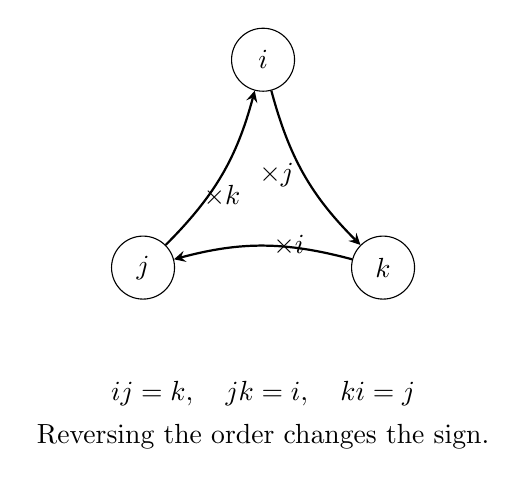
\begin{tikzpicture}[scale=1.1,>=stealth]
\node[circle,draw,minimum size=8mm] (i) at (90:1.6) {\(i\)};
\node[circle,draw,minimum size=8mm] (j) at (210:1.6) {\(j\)};
\node[circle,draw,minimum size=8mm] (k) at (330:1.6) {\(k\)};

\draw[->,thick] (i) to[bend right=15] node[left]{\(\times j\)} (k);
\draw[->,thick] (j) to[bend right=15] node[below]{\(\times k\)} (i);
\draw[->,thick] (k) to[bend right=15] node[right]{\(\times i\)} (j);

\node at (0,-2.25) {\(ij=k,\quad jk=i,\quad ki=j\)};
\node at (0,-2.75) {Reversing the order changes the sign.};
\end{tikzpicture}
\end{center}

Thus

\[ ji=-k,\qquad kj=-i,\qquad ik=-j. \]

%%%%%%%%%%%%%%%%%%%%%%%%%%%%%%%%%%%%%%%%%%%%%%%%%%%%%%%%%%%%
\subsection{Quaternion Conjugation and Norm}
\label{subsec:quaternion-conjugation}
%%%%%%%%%%%%%%%%%%%%%%%%%%%%%%%%%%%%%%%%%%%%%%%%%%%%%%%%%%%%

For

\[ q=a+bi+cj+dk, \]

define the conjugate

\[ \overline q=a-bi-cj-dk. \]

Then

\[ q\overline q=\overline q q=a^2+b^2+c^2+d^2. \]

For \(q\neq0\),

\[ q^{-1}=\frac{\overline q}{a^2+b^2+c^2+d^2}. \]

Thus every nonzero quaternion is invertible.

This proves that \(\mathbb H\) is a division ring.

%%%%%%%%%%%%%%%%%%%%%%%%%%%%%%%%%%%%%%%%%%%%%%%%%%%%%%%%%%%%
\subsection{Simple Rings}
\label{subsec:simple-rings}
%%%%%%%%%%%%%%%%%%%%%%%%%%%%%%%%%%%%%%%%%%%%%%%%%%%%%%%%%%%%

\begin{definitionbox}{Simple Ring}
A nonzero ring \(R\) is \emph{simple} if its only two-sided ideals are
\[ (0)\qquad\text{and}\qquad R. \]
\end{definitionbox}

Simple rings are building blocks in noncommutative ring theory.

Notice that simplicity concerns two-sided ideals. A simple ring may still
possess many nontrivial left or right ideals.

%%%%%%%%%%%%%%%%%%%%%%%%%%%%%%%%%%%%%%%%%%%%%%%%%%%%%%%%%%%%
\subsection{Matrix Rings Are Simple}
\label{subsec:matrix-rings-simple}
%%%%%%%%%%%%%%%%%%%%%%%%%%%%%%%%%%%%%%%%%%%%%%%%%%%%%%%%%%%%

If \(D\) is a division ring, then

\[ M_n(D) \]

is a simple ring.

For \(n>1\), it is generally not a division ring because nonzero singular
matrices are not invertible.

Thus

\[ \text{simple ring}\not\Rightarrow\text{division ring}. \]

Matrix rings demonstrate why the study of two-sided ideals alone does not
capture all noncommutative structure.

%%%%%%%%%%%%%%%%%%%%%%%%%%%%%%%%%%%%%%%%%%%%%%%%%%%%%%%%%%%%
\subsection{Minimal Left Ideals}
\label{subsec:minimal-left-ideals}
%%%%%%%%%%%%%%%%%%%%%%%%%%%%%%%%%%%%%%%%%%%%%%%%%%%%%%%%%%%%

A nonzero left ideal \(L\subseteq R\) is \emph{minimal} if it contains no
nonzero proper left ideal.

Thus if

\[ 0\neq K\subseteq L \]

and \(K\) is a left ideal, then

\[ K=L. \]

Minimal left ideals often behave like irreducible pieces of the regular
module \(R\).

%%%%%%%%%%%%%%%%%%%%%%%%%%%%%%%%%%%%%%%%%%%%%%%%%%%%%%%%%%%%
\subsection{Simple Modules}
\label{subsec:simple-modules}
%%%%%%%%%%%%%%%%%%%%%%%%%%%%%%%%%%%%%%%%%%%%%%%%%%%%%%%%%%%%

\begin{definitionbox}{Simple Module}
A nonzero left \(R\)-module \(M\) is \emph{simple} if its only submodules are
\[ 0\qquad\text{and}\qquad M. \]
\end{definitionbox}

Simple modules play a role analogous to prime building blocks.

A minimal left ideal of \(R\) is a simple left \(R\)-module.

%%%%%%%%%%%%%%%%%%%%%%%%%%%%%%%%%%%%%%%%%%%%%%%%%%%%%%%%%%%%
\subsection{The Regular Module}
\label{subsec:regular-module}
%%%%%%%%%%%%%%%%%%%%%%%%%%%%%%%%%%%%%%%%%%%%%%%%%%%%%%%%%%%%

Every ring \(R\) can act on itself by left multiplication.

This produces the left regular module

\[ {}_RR. \]

The notation

\[ {}_RR \]

indicates that \(R\) is being regarded as a left module over itself.

Similarly,

\[ R_R \]

denotes \(R\) as a right module over itself.

The submodules of \({}_RR\) are exactly the left ideals of \(R\).

The submodules of \(R_R\) are exactly the right ideals.

%%%%%%%%%%%%%%%%%%%%%%%%%%%%%%%%%%%%%%%%%%%%%%%%%%%%%%%%%%%%
\subsection{Ring Theory Through Module Theory}
\label{subsec:ring-through-module-theory}
%%%%%%%%%%%%%%%%%%%%%%%%%%%%%%%%%%%%%%%%%%%%%%%%%%%%%%%%%%%%

This gives an important translation:

\begin{center}
\begin{tabularx}{0.88\textwidth}{@{}XX@{}}
\toprule
\textbf{Ring Language} & \textbf{Module Language}\\
\midrule
Left ideal of \(R\) & Submodule of \({}_RR\)\\
Right ideal of \(R\) & Submodule of \(R_R\)\\
Minimal left ideal & Simple submodule of \({}_RR\)\\
Ascending chains of left ideals & Ascending chains of submodules\\
Descending chains of left ideals & Descending chains of submodules\\
\bottomrule
\end{tabularx}
\end{center}

Much of advanced noncommutative algebra therefore studies rings by studying
their module categories.

%%%%%%%%%%%%%%%%%%%%%%%%%%%%%%%%%%%%%%%%%%%%%%%%%%%%%%%%%%%%
\subsection{Chain Conditions}
\label{subsec:noncommutative-chain-conditions}
%%%%%%%%%%%%%%%%%%%%%%%%%%%%%%%%%%%%%%%%%%%%%%%%%%%%%%%%%%%%

As in commutative algebra, chain conditions control infinite growth.

A ring satisfies the ascending chain condition on left ideals if every chain

\[ I_1\subseteq I_2\subseteq I_3\subseteq\cdots \]

eventually stabilizes.

It satisfies the descending chain condition on left ideals if every chain

\[ I_1\supseteq I_2\supseteq I_3\supseteq\cdots \]

eventually stabilizes.

%%%%%%%%%%%%%%%%%%%%%%%%%%%%%%%%%%%%%%%%%%%%%%%%%%%%%%%%%%%%
\subsection{Left and Right Noetherian Rings}
\label{subsec:left-right-noetherian}
%%%%%%%%%%%%%%%%%%%%%%%%%%%%%%%%%%%%%%%%%%%%%%%%%%%%%%%%%%%%

\begin{definitionbox}{Left Noetherian Ring}
A ring \(R\) is \emph{left Noetherian} if it satisfies the ascending chain
condition on left ideals.
\end{definitionbox}

Equivalently, every left ideal is finitely generated as a left ideal.

Similarly, \(R\) is \emph{right Noetherian} if every right ideal is finitely
generated.

In a noncommutative ring,

\[ \text{left Noetherian} \]

and

\[ \text{right Noetherian} \]

are conceptually distinct conditions.

%%%%%%%%%%%%%%%%%%%%%%%%%%%%%%%%%%%%%%%%%%%%%%%%%%%%%%%%%%%%
\subsection{Artinian Rings}
\label{subsec:artinian-rings}
%%%%%%%%%%%%%%%%%%%%%%%%%%%%%%%%%%%%%%%%%%%%%%%%%%%%%%%%%%%%

\begin{definitionbox}{Left Artinian Ring}
A ring \(R\) is \emph{left Artinian} if every descending chain of left ideals
eventually stabilizes.
\end{definitionbox}

Similarly, one defines right Artinian rings using right ideals.

The terminology honors Emil Artin.

Noetherian conditions prevent infinite upward growth, while Artinian
conditions prevent infinite downward refinement.

\begin{center}
\begin{tikzpicture}[
    node distance=12mm and 20mm,
    box/.style={draw,rounded corners,align=center,inner sep=5pt},
    >=stealth
]
\node[box] (chain) {Chains of ideals};
\node[box,below left=of chain] (noeth) {Ascending chains\\stabilize};
\node[box,below right=of chain] (artin) {Descending chains\\stabilize};
\node[box,below=of noeth] (N) {Noetherian};
\node[box,below=of artin] (A) {Artinian};

\draw[->,thick] (chain)--(noeth);
\draw[->,thick] (chain)--(artin);
\draw[->,thick] (noeth)--(N);
\draw[->,thick] (artin)--(A);
\end{tikzpicture}
\end{center}

%%%%%%%%%%%%%%%%%%%%%%%%%%%%%%%%%%%%%%%%%%%%%%%%%%%%%%%%%%%%
\subsection{The Jacobson Radical}
\label{subsec:jacobson-radical}
%%%%%%%%%%%%%%%%%%%%%%%%%%%%%%%%%%%%%%%%%%%%%%%%%%%%%%%%%%%%

The Jacobson radical is one of the most important radicals in
noncommutative algebra.

\begin{definitionbox}{Jacobson Radical}
For a ring \(R\), the \emph{Jacobson radical}, denoted
\[ J(R), \]
is the intersection of all maximal left ideals of \(R\).
\end{definitionbox}

The notation

\[ J(R) \]

is read ``the Jacobson radical of \(R\).''

Although the definition uses maximal left ideals, \(J(R)\) is a two-sided
ideal.

%%%%%%%%%%%%%%%%%%%%%%%%%%%%%%%%%%%%%%%%%%%%%%%%%%%%%%%%%%%%
\subsection{Interpreting the Jacobson Radical}
\label{subsec:jacobson-radical-meaning}
%%%%%%%%%%%%%%%%%%%%%%%%%%%%%%%%%%%%%%%%%%%%%%%%%%%%%%%%%%%%

The Jacobson radical can be viewed as a portion of the ring that becomes
invisible to simple modules.

One characterization is

\[ J(R)=\bigcap_{M\text{ simple}}\Ann_R(M), \]

with the intersection taken over simple left \(R\)-modules.

Thus elements of \(J(R)\) act as zero on every simple left module.

\begin{conceptbox}
The Jacobson radical measures a kind of ``non-semisimple remainder'' of a
ring.

Passing to
\[ R/J(R) \]
often reveals a cleaner semisimple structure.
\end{conceptbox}

%%%%%%%%%%%%%%%%%%%%%%%%%%%%%%%%%%%%%%%%%%%%%%%%%%%%%%%%%%%%
\subsection{Jacobson Radical of a Field}
\label{subsec:jacobson-radical-field}
%%%%%%%%%%%%%%%%%%%%%%%%%%%%%%%%%%%%%%%%%%%%%%%%%%%%%%%%%%%%

If \(F\) is a field, its only maximal ideal is

\[ (0). \]

Therefore,

\[ J(F)=(0). \]

Likewise, if \(D\) is a division ring,

\[ J(D)=0. \]

%%%%%%%%%%%%%%%%%%%%%%%%%%%%%%%%%%%%%%%%%%%%%%%%%%%%%%%%%%%%
\subsection{Jacobson Radical of a Matrix Ring}
\label{subsec:jacobson-radical-matrix}
%%%%%%%%%%%%%%%%%%%%%%%%%%%%%%%%%%%%%%%%%%%%%%%%%%%%%%%%%%%%

A fundamental compatibility property is

\[ J(M_n(R))=M_n(J(R)). \]

In particular, if \(F\) is a field,

\[ J(M_n(F))=0. \]

This is consistent with the semisimple nature of matrix rings over division
rings.

%%%%%%%%%%%%%%%%%%%%%%%%%%%%%%%%%%%%%%%%%%%%%%%%%%%%%%%%%%%%
\subsection{Semisimple Modules}
\label{subsec:semisimple-modules}
%%%%%%%%%%%%%%%%%%%%%%%%%%%%%%%%%%%%%%%%%%%%%%%%%%%%%%%%%%%%

\begin{definitionbox}{Semisimple Module}
An \(R\)-module \(M\) is \emph{semisimple} if it can be expressed as a direct
sum of simple submodules.
\end{definitionbox}

Thus

\[ M\cong\bigoplus_{\alpha\in A}M_\alpha, \]

where each \(M_\alpha\) is simple.

The symbol

\[ \bigoplus \]

denotes a direct sum and is read ``direct sum.''

%%%%%%%%%%%%%%%%%%%%%%%%%%%%%%%%%%%%%%%%%%%%%%%%%%%%%%%%%%%%
\subsection{Semisimple Rings}
\label{subsec:semisimple-rings}
%%%%%%%%%%%%%%%%%%%%%%%%%%%%%%%%%%%%%%%%%%%%%%%%%%%%%%%%%%%%

\begin{definitionbox}{Semisimple Ring}
A ring \(R\) is \emph{semisimple} if the left regular module
\[ {}_RR \]
is semisimple.
\end{definitionbox}

For rings with identity, left and right semisimplicity ultimately coincide.

Semisimple rings have exceptionally rigid structure.

%%%%%%%%%%%%%%%%%%%%%%%%%%%%%%%%%%%%%%%%%%%%%%%%%%%%%%%%%%%%
\subsection{The Artin--Wedderburn Theorem}
\label{subsec:artin-wedderburn}
%%%%%%%%%%%%%%%%%%%%%%%%%%%%%%%%%%%%%%%%%%%%%%%%%%%%%%%%%%%%

One of the central classification theorems of noncommutative algebra is the
Artin--Wedderburn theorem.

\begin{theorem}[Artin--Wedderburn]
A semisimple Artinian ring is isomorphic to a finite direct product of full
matrix rings over division rings:
\[ R\cong M_{n_1}(D_1)\times\cdots\times M_{n_k}(D_k), \]
where each \(D_i\) is a division ring.
\end{theorem}

This theorem says that semisimple rings are assembled from highly concrete
building blocks.

%%%%%%%%%%%%%%%%%%%%%%%%%%%%%%%%%%%%%%%%%%%%%%%%%%%%%%%%%%%%
\subsection{Visualizing Artin--Wedderburn}
\label{subsec:artin-wedderburn-visual}
%%%%%%%%%%%%%%%%%%%%%%%%%%%%%%%%%%%%%%%%%%%%%%%%%%%%%%%%%%%%

\begin{center}
\begin{tikzpicture}[
    node distance=11mm and 10mm,
    box/.style={draw,rounded corners,align=center,inner sep=5pt,font=\small},
    >=stealth
]
\node[box] (R) {Semisimple\\Artinian ring \(R\)};
\node[box,below=of R] (decomp) {Finite product};
\node[box,below left=of decomp] (M1) {\(M_{n_1}(D_1)\)};
\node[box,below=of decomp] (M2) {\(\cdots\)};
\node[box,below right=of decomp] (Mk) {\(M_{n_k}(D_k)\)};

\draw[->,thick] (R)--node[right]{classification}(decomp);
\draw[->,thick] (decomp)--(M1);
\draw[->,thick] (decomp)--(M2);
\draw[->,thick] (decomp)--(Mk);
\end{tikzpicture}
\end{center}

The theorem reduces an abstract structural question to matrix algebra over
division rings.

%%%%%%%%%%%%%%%%%%%%%%%%%%%%%%%%%%%%%%%%%%%%%%%%%%%%%%%%%%%%
\subsection{Simple Artinian Rings}
\label{subsec:simple-artinian-rings}
%%%%%%%%%%%%%%%%%%%%%%%%%%%%%%%%%%%%%%%%%%%%%%%%%%%%%%%%%%%%

An important special case states:

\begin{theorem}
Every simple Artinian ring is isomorphic to
\[ M_n(D) \]
for some division ring \(D\) and positive integer \(n\).
\end{theorem}

Thus full matrix rings over division rings are precisely the simple
Artinian rings.

%%%%%%%%%%%%%%%%%%%%%%%%%%%%%%%%%%%%%%%%%%%%%%%%%%%%%%%%%%%%
\subsection{Group Algebras}
\label{subsec:group-algebras}
%%%%%%%%%%%%%%%%%%%%%%%%%%%%%%%%%%%%%%%%%%%%%%%%%%%%%%%%%%%%

Noncommutative rings arise naturally from groups.

Let \(F\) be a field and \(G\) a group.

\begin{definitionbox}{Group Algebra}
The \emph{group algebra} \(F[G]\) consists of finite formal sums
\[ \sum_{g\in G}a_g g,\qquad a_g\in F, \]
with multiplication induced by the group operation and distributivity.
\end{definitionbox}

The notation

\[ F[G] \]

is read ``the group algebra of \(G\) over \(F\).''

If \(G\) is nonabelian, then \(F[G]\) is generally noncommutative.

%%%%%%%%%%%%%%%%%%%%%%%%%%%%%%%%%%%%%%%%%%%%%%%%%%%%%%%%%%%%
\subsection{Multiplication in a Group Algebra}
\label{subsec:group-algebra-multiplication}
%%%%%%%%%%%%%%%%%%%%%%%%%%%%%%%%%%%%%%%%%%%%%%%%%%%%%%%%%%%%

Suppose

\[ x=\sum_{g\in G}a_gg,\qquad y=\sum_{h\in G}b_hh. \]

Then

\[ xy=\sum_{g,h}a_gb_h(gh). \]

The multiplication rule comes directly from the group multiplication.

Therefore, if

\[ gh\neq hg, \]

then the corresponding basis elements also fail to commute inside the group
algebra.

%%%%%%%%%%%%%%%%%%%%%%%%%%%%%%%%%%%%%%%%%%%%%%%%%%%%%%%%%%%%
\subsection{Group Algebras and Representation Theory}
\label{subsec:group-algebras-representations}
%%%%%%%%%%%%%%%%%%%%%%%%%%%%%%%%%%%%%%%%%%%%%%%%%%%%%%%%%%%%

Representations of \(G\) over \(F\) can be interpreted as modules over the
group algebra \(F[G]\).

This creates a fundamental bridge:

\begin{center}
\begin{tikzpicture}[
    node distance=16mm,
    box/.style={draw,rounded corners,align=center,inner sep=6pt},
    >=stealth
]
\node[box] (group) {Group \(G\)};
\node[box,right=of group] (alg) {Group algebra\\\(F[G]\)};
\node[box,right=of alg] (mod) {\(F[G]\)-modules};
\node[box,below=of mod] (rep) {Representations\\of \(G\)};

\draw[->,thick] (group)--(alg);
\draw[->,thick] (alg)--(mod);
\draw[<->,thick] (mod)--(rep);
\end{tikzpicture}
\end{center}

This relationship will be developed canonically in
\cref{sec:representation-theory}.

%%%%%%%%%%%%%%%%%%%%%%%%%%%%%%%%%%%%%%%%%%%%%%%%%%%%%%%%%%%%
\subsection{Maschke's Theorem}
\label{subsec:maschke-preview}
%%%%%%%%%%%%%%%%%%%%%%%%%%%%%%%%%%%%%%%%%%%%%%%%%%%%%%%%%%%%

A major result connects finite groups with semisimple rings.

\begin{theorem}[Maschke's Theorem]
Let \(G\) be a finite group and \(F\) a field such that
\[ \operatorname{char}(F)\nmid |G|. \]
Then the group algebra
\[ F[G] \]
is semisimple.
\end{theorem}

The notation

\[ \operatorname{char}(F) \]

means the characteristic of \(F\) and is read ``the characteristic of
\(F\).''

The symbol

\[ \nmid \]

is read ``does not divide.''

Thus the condition is read:

``the characteristic of \(F\) does not divide the order of \(G\).''

%%%%%%%%%%%%%%%%%%%%%%%%%%%%%%%%%%%%%%%%%%%%%%%%%%%%%%%%%%%%
\subsection{Free Associative Algebras}
\label{subsec:free-associative-algebras}
%%%%%%%%%%%%%%%%%%%%%%%%%%%%%%%%%%%%%%%%%%%%%%%%%%%%%%%%%%%%

Ordinary polynomial rings satisfy

\[ xy=yx. \]

To construct a polynomial-like algebra where variables do not commute, one
uses a free associative algebra.

\begin{definitionbox}{Free Associative Algebra}
Let \(F\) be a field. The \emph{free associative algebra} on generators
\(x_1,\ldots,x_n\) is denoted
\[ F\langle x_1,\ldots,x_n\rangle. \]
Its elements are finite \(F\)-linear combinations of words in the
generators, with multiplication given by concatenation.
\end{definitionbox}

The angle-bracket notation

\[ F\langle x,y\rangle \]

is read ``the free associative algebra over \(F\) on \(x\) and \(y\).''

%%%%%%%%%%%%%%%%%%%%%%%%%%%%%%%%%%%%%%%%%%%%%%%%%%%%%%%%%%%%
\subsection{Words in Noncommuting Variables}
\label{subsec:noncommuting-words}
%%%%%%%%%%%%%%%%%%%%%%%%%%%%%%%%%%%%%%%%%%%%%%%%%%%%%%%%%%%%

In

\[ F\langle x,y\rangle, \]

the monomials

\[ xy\qquad\text{and}\qquad yx \]

are distinct.

Likewise,

\[ xxy,\qquad xyx,\qquad yxx \]

are different words.

Thus multiplication remembers order.

\begin{center}
\begin{tikzpicture}[
    node distance=8mm,
    every node/.style={font=\small},
    >=stealth
]
\node (start) {\(1\)};
\node[below left=of start] (x) {\(x\)};
\node[below right=of start] (y) {\(y\)};
\node[below left=of x] (xx) {\(x^2\)};
\node[below right=of x] (xy) {\(xy\)};
\node[below left=of y] (yx) {\(yx\)};
\node[below right=of y] (yy) {\(y^2\)};

\draw[->] (start)--(x);
\draw[->] (start)--(y);
\draw[->] (x)--(xx);
\draw[->] (x)--(xy);
\draw[->] (y)--(yx);
\draw[->] (y)--(yy);
\end{tikzpicture}
\end{center}

The branching reflects the growing number of distinct words.

%%%%%%%%%%%%%%%%%%%%%%%%%%%%%%%%%%%%%%%%%%%%%%%%%%%%%%%%%%%%
\subsection{Noncommutative Polynomial Relations}
\label{subsec:noncommutative-relations}
%%%%%%%%%%%%%%%%%%%%%%%%%%%%%%%%%%%%%%%%%%%%%%%%%%%%%%%%%%%%

Many important algebras are formed by starting with a free associative
algebra and imposing relations.

For example,

\[ A=F\langle x,y\rangle/(yx-xy-1). \]

Inside this quotient,

\[ yx-xy=1. \]

Equivalently,

\[ yx=xy+1. \]

This is a fundamentally noncommutative relation.

%%%%%%%%%%%%%%%%%%%%%%%%%%%%%%%%%%%%%%%%%%%%%%%%%%%%%%%%%%%%
\subsection{The Weyl Algebra}
\label{subsec:weyl-algebra}
%%%%%%%%%%%%%%%%%%%%%%%%%%%%%%%%%%%%%%%%%%%%%%%%%%%%%%%%%%%%

The first Weyl algebra over a field \(F\) can be presented as

\[ A_1(F)=F\langle x,\partial\rangle/(\partial x-x\partial-1). \]

The symbol

\[ \partial \]

is the partial-derivative symbol, pronounced ``partial.''

The defining relation is

\[ \partial x-x\partial=1. \]

This mirrors the operator identity

\[ \frac{d}{dx}(xf)-x\frac{df}{dx}=f. \]

Thus noncommutative algebra naturally models differential operators.

%%%%%%%%%%%%%%%%%%%%%%%%%%%%%%%%%%%%%%%%%%%%%%%%%%%%%%%%%%%%
\subsection{Operator Interpretation of the Weyl Relation}
\label{subsec:weyl-operator-interpretation}
%%%%%%%%%%%%%%%%%%%%%%%%%%%%%%%%%%%%%%%%%%%%%%%%%%%%%%%%%%%%

Let \(X\) denote multiplication by \(x\),

\[ X(f)=xf, \]

and let \(D\) denote differentiation,

\[ D(f)=f'. \]

Then

\[ DX(f)=D(xf)=f+xf' \]

while

\[ XD(f)=xf'. \]

Therefore,

\[ (DX-XD)(f)=f. \]

Hence

\[ DX-XD=I. \]

In commutator notation,

\[ [D,X]=I. \]

This is a concrete example of noncommutativity encoding a mathematical
operation.

%%%%%%%%%%%%%%%%%%%%%%%%%%%%%%%%%%%%%%%%%%%%%%%%%%%%%%%%%%%%
\subsection{Algebras over a Field}
\label{subsec:noncommutative-algebras-over-field}
%%%%%%%%%%%%%%%%%%%%%%%%%%%%%%%%%%%%%%%%%%%%%%%%%%%%%%%%%%%%

An \(F\)-algebra combines vector-space structure with compatible ring
multiplication.

When multiplication is not required to commute, examples include:

\[ M_n(F),\qquad F[G],\qquad F\langle x_1,\ldots,x_n\rangle,\qquad A_1(F). \]

These objects can be studied simultaneously using both linear algebra and
ring theory.

%%%%%%%%%%%%%%%%%%%%%%%%%%%%%%%%%%%%%%%%%%%%%%%%%%%%%%%%%%%%
\subsection{Bimodules}
\label{subsec:bimodules}
%%%%%%%%%%%%%%%%%%%%%%%%%%%%%%%%%%%%%%%%%%%%%%%%%%%%%%%%%%%%

Some modules carry compatible actions from both sides.

\begin{definitionbox}{Bimodule}
Let \(R\) and \(S\) be rings. An \((R,S)\)-\emph{bimodule} \(M\) is both a
left \(R\)-module and a right \(S\)-module such that
\[ (rm)s=r(ms) \]
for all \(r\in R\), \(m\in M\), and \(s\in S\).
\end{definitionbox}

The notation

\[ {}_RM_S \]

is often used to emphasize both actions.

Bimodules become important in tensor products, representation theory,
homological algebra, and equivalences between module categories.

%%%%%%%%%%%%%%%%%%%%%%%%%%%%%%%%%%%%%%%%%%%%%%%%%%%%%%%%%%%%
\subsection{Central Algebras}
\label{subsec:central-algebras}
%%%%%%%%%%%%%%%%%%%%%%%%%%%%%%%%%%%%%%%%%%%%%%%%%%%%%%%%%%%%

Let \(F\) be a field and \(A\) an \(F\)-algebra.

The algebra \(A\) is called \emph{central over \(F\)} when

\[ Z(A)=F, \]

where \(F\) is identified with scalar multiples of the identity.

For example,

\[ Z(M_n(F))=\{\lambda I_n:\lambda\in F\}, \]

so \(M_n(F)\) is central over \(F\).

%%%%%%%%%%%%%%%%%%%%%%%%%%%%%%%%%%%%%%%%%%%%%%%%%%%%%%%%%%%%
\subsection{Central Simple Algebras}
\label{subsec:central-simple-algebras}
%%%%%%%%%%%%%%%%%%%%%%%%%%%%%%%%%%%%%%%%%%%%%%%%%%%%%%%%%%%%

\begin{definitionbox}{Central Simple Algebra}
An \(F\)-algebra \(A\) is a \emph{central simple algebra} if:
\begin{enumerate}
    \item \(A\) is finite-dimensional over \(F\);
    \item \(A\) is simple as a ring;
    \item \(Z(A)=F\).
\end{enumerate}
\end{definitionbox}

Matrix algebras

\[ M_n(F) \]

are fundamental examples.

The theory of central simple algebras connects noncommutative algebra with
field theory, number theory, and geometry.

%%%%%%%%%%%%%%%%%%%%%%%%%%%%%%%%%%%%%%%%%%%%%%%%%%%%%%%%%%%%
\subsection{Polynomial Identities}
\label{subsec:polynomial-identities}
%%%%%%%%%%%%%%%%%%%%%%%%%%%%%%%%%%%%%%%%%%%%%%%%%%%%%%%%%%%%

A noncommutative ring may satisfy polynomial identities even though its
elements do not commute.

For example, matrix rings satisfy important identities involving
noncommuting variables.

This motivates the study of \emph{PI-rings}, where ``PI'' stands for
``polynomial identity.''

The subject lies between commutative algebra and completely unrestricted
noncommutative algebra.

%%%%%%%%%%%%%%%%%%%%%%%%%%%%%%%%%%%%%%%%%%%%%%%%%%%%%%%%%%%%
\subsection{Noncommutative Localization}
\label{subsec:noncommutative-localization}
%%%%%%%%%%%%%%%%%%%%%%%%%%%%%%%%%%%%%%%%%%%%%%%%%%%%%%%%%%%%

In commutative algebra, a multiplicatively closed set \(S\) can usually be
localized directly.

In a noncommutative ring, expressions such as

\[ s^{-1}r \qquad\text{and}\qquad rs^{-1} \]

need not behave identically.

Therefore constructing rings of fractions requires additional compatibility
conditions.

One important framework uses \emph{Ore conditions}.

%%%%%%%%%%%%%%%%%%%%%%%%%%%%%%%%%%%%%%%%%%%%%%%%%%%%%%%%%%%%
\subsection{Ore Conditions: Conceptual Preview}
\label{subsec:ore-condition-preview}
%%%%%%%%%%%%%%%%%%%%%%%%%%%%%%%%%%%%%%%%%%%%%%%%%%%%%%%%%%%%

The Ore conditions ensure that denominators can be moved past numerators in
a controlled manner.

Schematically, one seeks common multiples allowing expressions such as

\[ rs^{-1} \]

to interact consistently with noncommutative multiplication.

\begin{conceptbox}
Commutative localization works smoothly because
\[ rs=sr. \]

When multiplication is noncommutative, the placement of denominators matters.
Ore localization supplies conditions under which a workable theory of
fractions can still be constructed.
\end{conceptbox}

The full technical development belongs to more advanced noncommutative ring
theory.

%%%%%%%%%%%%%%%%%%%%%%%%%%%%%%%%%%%%%%%%%%%%%%%%%%%%%%%%%%%%
\subsection{Prime Ideals in Noncommutative Rings}
\label{subsec:noncommutative-prime-ideals}
%%%%%%%%%%%%%%%%%%%%%%%%%%%%%%%%%%%%%%%%%%%%%%%%%%%%%%%%%%%%

The commutative condition

\[ ab\in\mathfrak p\implies a\in\mathfrak p\text{ or }b\in\mathfrak p \]

does not transfer perfectly to arbitrary noncommutative rings.

A common two-sided definition is:

\begin{definitionbox}{Prime Ring Ideal}
A proper two-sided ideal \(P\) of \(R\) is \emph{prime} if for two-sided
ideals \(I,J\trianglelefteq R\),
\[ IJ\subseteq P\implies I\subseteq P\text{ or }J\subseteq P. \]
\end{definitionbox}

Equivalently,

\[ R/P \]

is a prime ring.

This illustrates an important principle: definitions from commutative
algebra may require structural modification in the noncommutative setting.

%%%%%%%%%%%%%%%%%%%%%%%%%%%%%%%%%%%%%%%%%%%%%%%%%%%%%%%%%%%%
\subsection{Prime Rings}
\label{subsec:prime-rings}
%%%%%%%%%%%%%%%%%%%%%%%%%%%%%%%%%%%%%%%%%%%%%%%%%%%%%%%%%%%%

\begin{definitionbox}{Prime Ring}
A nonzero ring \(R\) is \emph{prime} if
\[ aRb=0 \]
implies
\[ a=0\quad\text{or}\quad b=0. \]
\end{definitionbox}

Here

\[ aRb=\{arb:r\in R\}. \]

The condition is stronger than merely testing a single product \(ab\).

Every simple ring is prime.

%%%%%%%%%%%%%%%%%%%%%%%%%%%%%%%%%%%%%%%%%%%%%%%%%%%%%%%%%%%%
\subsection{Domains in the Noncommutative Setting}
\label{subsec:noncommutative-domains}
%%%%%%%%%%%%%%%%%%%%%%%%%%%%%%%%%%%%%%%%%%%%%%%%%%%%%%%%%%%%

A noncommutative domain is typically a nonzero ring satisfying

\[ ab=0\implies a=0\text{ or }b=0. \]

Commutativity is not required.

For example, every division ring is a domain.

However, many familiar equivalences from commutative integral domains must
be reconsidered when multiplication does not commute.

%%%%%%%%%%%%%%%%%%%%%%%%%%%%%%%%%%%%%%%%%%%%%%%%%%%%%%%%%%%%
\subsection{Homomorphisms}
\label{subsec:noncommutative-homomorphisms}
%%%%%%%%%%%%%%%%%%%%%%%%%%%%%%%%%%%%%%%%%%%%%%%%%%%%%%%%%%%%

A ring homomorphism

\[ \varphi:R\to S \]

must preserve multiplication in the given order:

\[ \varphi(ab)=\varphi(a)\varphi(b). \]

One cannot replace the right side with

\[ \varphi(b)\varphi(a) \]

unless additional commutativity is available.

The kernel

\[ \Ker(\varphi) \]

is a two-sided ideal of \(R\).

%%%%%%%%%%%%%%%%%%%%%%%%%%%%%%%%%%%%%%%%%%%%%%%%%%%%%%%%%%%%
\subsection{The First Isomorphism Theorem}
\label{subsec:noncommutative-first-isomorphism}
%%%%%%%%%%%%%%%%%%%%%%%%%%%%%%%%%%%%%%%%%%%%%%%%%%%%%%%%%%%%

The familiar ring isomorphism theorem remains valid.

\begin{theorem}[First Isomorphism Theorem for Rings]
Let
\[ \varphi:R\to S \]
be a ring homomorphism. Then
\[ R/\Ker(\varphi)\cong\Image(\varphi). \]
\end{theorem}

The kernel is automatically two-sided, so the quotient ring is well defined.

\begin{center}
\begin{tikzcd}
R \arrow[r,"\varphi"] \arrow[d,"\pi"'] &
\Image(\varphi) \\
R/\Ker(\varphi) \arrow[ur,"\cong"']
\end{tikzcd}
\end{center}

Here \(\pi\) denotes the canonical quotient map.

%%%%%%%%%%%%%%%%%%%%%%%%%%%%%%%%%%%%%%%%%%%%%%%%%%%%%%%%%%%%
\subsection{Inner Automorphisms}
\label{subsec:inner-automorphisms-rings}
%%%%%%%%%%%%%%%%%%%%%%%%%%%%%%%%%%%%%%%%%%%%%%%%%%%%%%%%%%%%

Noncommutative rings possess natural automorphisms arising from units.

Let \(u\in R^\times\).

Define

\[ \varphi_u(r)=uru^{-1}. \]

Then \(\varphi_u\) is a ring automorphism called an \emph{inner
automorphism}.

Conjugation can change an element while preserving substantial structural
information.

%%%%%%%%%%%%%%%%%%%%%%%%%%%%%%%%%%%%%%%%%%%%%%%%%%%%%%%%%%%%
\subsection{Conjugation and the Center}
\label{subsec:conjugation-center}
%%%%%%%%%%%%%%%%%%%%%%%%%%%%%%%%%%%%%%%%%%%%%%%%%%%%%%%%%%%%

An element \(z\in R\) belongs to the center exactly when it is unchanged by
every inner automorphism:

\[ uzu^{-1}=z \]

for every unit \(u\), under appropriate hypotheses on the units available.

Thus central elements are precisely those insensitive to the order effects
represented by conjugation.

%%%%%%%%%%%%%%%%%%%%%%%%%%%%%%%%%%%%%%%%%%%%%%%%%%%%%%%%%%%%
\subsection{Morita Equivalence: A Preview}
\label{subsec:morita-equivalence-preview}
%%%%%%%%%%%%%%%%%%%%%%%%%%%%%%%%%%%%%%%%%%%%%%%%%%%%%%%%%%%%

Two rings may be very different as rings while having essentially equivalent
module theories.

This phenomenon is called \emph{Morita equivalence}.

The standard example is

\[ R\qquad\text{and}\qquad M_n(R). \]

Although these rings are generally not isomorphic,

\[ R\not\cong M_n(R), \]

their module categories are closely related.

\begin{center}
\begin{tikzpicture}[
    node distance=18mm,
    box/.style={draw,rounded corners,align=center,inner sep=6pt},
    >=stealth
]
\node[box] (R) {Ring \(R\)};
\node[box,right=of R] (Mn) {Matrix ring\\\(M_n(R)\)};
\node[box,below=of R] (RM) {\(R\)-modules};
\node[box,below=of Mn] (MM) {\(M_n(R)\)-modules};

\draw[->,thick] (R)--(RM);
\draw[->,thick] (Mn)--(MM);
\draw[<->,thick,dashed] (RM)--node[below]{equivalent categories}(MM);
\end{tikzpicture}
\end{center}

Morita theory emphasizes that module categories can sometimes reveal more
structural information than the literal presentation of a ring.

%%%%%%%%%%%%%%%%%%%%%%%%%%%%%%%%%%%%%%%%%%%%%%%%%%%%%%%%%%%%
\subsection{Worked Example: A Left Ideal}
\label{subsec:worked-left-ideal}
%%%%%%%%%%%%%%%%%%%%%%%%%%%%%%%%%%%%%%%%%%%%%%%%%%%%%%%%%%%%

\begin{workedexamplebox}{Testing a Left Ideal in \(M_2(F)\)}

Let

\[ I=\left\{
\begin{pmatrix}
a&0\\
b&0
\end{pmatrix}:a,b\in F
\right\}. \]

Show that \(I\) is a left ideal of \(M_2(F)\).

\begin{tabularx}{\textwidth}{@{}>{\raggedright\arraybackslash}p{0.42\textwidth}X@{}}
Choose arbitrary elements. &
\(\displaystyle
A=\begin{pmatrix}p&q\\r&s\end{pmatrix},
\quad
X=\begin{pmatrix}a&0\\b&0\end{pmatrix}\)\\
Multiply on the left. &
\(\displaystyle
AX=
\begin{pmatrix}
pa+qb&0\\
ra+sb&0
\end{pmatrix}\)\\
Check the defining form. & The second column remains zero.\\
Conclude. & \(AX\in I\) for every \(A\in M_2(F)\) and \(X\in I\).
\end{tabularx}

\begin{answerbox}
\[ \boxed{I\text{ is a left ideal of }M_2(F).} \]
\end{answerbox}
\end{workedexamplebox}

%%%%%%%%%%%%%%%%%%%%%%%%%%%%%%%%%%%%%%%%%%%%%%%%%%%%%%%%%%%%
\subsection{Worked Example: Quaternion Noncommutativity}
\label{subsec:worked-quaternion}
%%%%%%%%%%%%%%%%%%%%%%%%%%%%%%%%%%%%%%%%%%%%%%%%%%%%%%%%%%%%

\begin{workedexamplebox}{Comparing \(ij\) and \(ji\)}

Use the quaternion multiplication rules to compare \(ij\) and \(ji\).

\begin{tabularx}{\textwidth}{@{}>{\raggedright\arraybackslash}p{0.42\textwidth}X@{}}
Use the forward cyclic product. & \(ij=k\)\\
Reverse the order. & \(ji=-k\)\\
Compare the results. & \(k\neq-k\)
\end{tabularx}

\begin{answerbox}
\[ \boxed{ij=k,\qquad ji=-k,\qquad ij\neq ji.} \]
\end{answerbox}
\end{workedexamplebox}

%%%%%%%%%%%%%%%%%%%%%%%%%%%%%%%%%%%%%%%%%%%%%%%%%%%%%%%%%%%%
\subsection{Worked Example: Center of \(M_2(F)\)}
\label{subsec:worked-center-matrix}
%%%%%%%%%%%%%%%%%%%%%%%%%%%%%%%%%%%%%%%%%%%%%%%%%%%%%%%%%%%%

\begin{workedexamplebox}{Recognizing Central Matrices}

Determine which of the following matrices must lie in the center of
\(M_2(\R)\):

\[ A=\begin{pmatrix}3&0\\0&3\end{pmatrix},\qquad
B=\begin{pmatrix}1&0\\0&2\end{pmatrix}. \]

\begin{tabularx}{\textwidth}{@{}>{\raggedright\arraybackslash}p{0.42\textwidth}X@{}}
Recognize \(A\). & \(A=3I_2\) is a scalar matrix.\\
Use the center theorem. & Every scalar matrix lies in \(Z(M_2(\R))\).\\
Recognize \(B\). & \(B\) is not a scalar matrix.\\
Apply the characterization. & \(B\notin Z(M_2(\R))\).
\end{tabularx}

\begin{answerbox}
\[ \boxed{A\in Z(M_2(\R)),\qquad B\notin Z(M_2(\R)).} \]
\end{answerbox}
\end{workedexamplebox}

%%%%%%%%%%%%%%%%%%%%%%%%%%%%%%%%%%%%%%%%%%%%%%%%%%%%%%%%%%%%
\subsection{Worked Example: Nilpotent and Idempotent Matrices}
\label{subsec:worked-nilpotent-idempotent}
%%%%%%%%%%%%%%%%%%%%%%%%%%%%%%%%%%%%%%%%%%%%%%%%%%%%%%%%%%%%

\begin{workedexamplebox}{Classifying Two Matrices}

Let

\[ N=\begin{pmatrix}0&1\\0&0\end{pmatrix},\qquad
E=\begin{pmatrix}1&0\\0&0\end{pmatrix}. \]

Classify \(N\) and \(E\).

\begin{tabularx}{\textwidth}{@{}>{\raggedright\arraybackslash}p{0.42\textwidth}X@{}}
Square \(N\). &
\(\displaystyle N^2=\begin{pmatrix}0&0\\0&0\end{pmatrix}\)\\
Classify \(N\). & \(N\) is nilpotent.\\
Square \(E\). &
\(\displaystyle E^2=\begin{pmatrix}1&0\\0&0\end{pmatrix}=E\)\\
Classify \(E\). & \(E\) is idempotent.
\end{tabularx}

\begin{answerbox}
\[ \boxed{N\text{ is nilpotent},\qquad E\text{ is idempotent}.} \]
\end{answerbox}
\end{workedexamplebox}

%%%%%%%%%%%%%%%%%%%%%%%%%%%%%%%%%%%%%%%%%%%%%%%%%%%%%%%%%%%%
\subsection{Noncommutative Algebra and Linear Algebra}
\label{subsec:noncommutative-linear-algebra}
%%%%%%%%%%%%%%%%%%%%%%%%%%%%%%%%%%%%%%%%%%%%%%%%%%%%%%%%%%%%

Linear algebra supplies some of the most important noncommutative examples.

Matrix multiplication,

\[ AB, \]

is composition of linear transformations.

Endomorphism rings,

\[ \End_F(V), \]

are naturally isomorphic to matrix rings after choosing a basis:

\[ \End_F(V)\cong M_n(F) \]

when

\[ \dim_F(V)=n. \]

Thus matrix algebra is not merely an example of noncommutative algebra; it is
one of its fundamental models.

%%%%%%%%%%%%%%%%%%%%%%%%%%%%%%%%%%%%%%%%%%%%%%%%%%%%%%%%%%%%
\subsection{Noncommutative Algebra and Group Theory}
\label{subsec:noncommutative-group-theory}
%%%%%%%%%%%%%%%%%%%%%%%%%%%%%%%%%%%%%%%%%%%%%%%%%%%%%%%%%%%%

Groups provide noncommutative multiplication whenever the group is
nonabelian.

From a group \(G\), one can construct:

\[ F[G], \]

its group algebra;

\[ \End_F(V), \]

through representations;

and matrix groups such as

\[ GL_n(F). \]

This creates a chain of connections:

\begin{center}
\begin{tikzpicture}[
    node distance=13mm,
    box/.style={draw,rounded corners,align=center,inner sep=5pt},
    >=stealth
]
\node[box] (G) {Group \(G\)};
\node[box,right=of G] (rep) {Representation};
\node[box,right=of rep] (matrix) {Matrices};
\node[box,below=of rep] (alg) {Group algebra \(F[G]\)};
\node[box,below=of matrix] (module) {Modules};

\draw[->,thick] (G)--(rep);
\draw[->,thick] (rep)--(matrix);
\draw[->,thick] (G)--(alg);
\draw[->,thick] (alg)--(module);
\draw[->,thick] (matrix)--(module);
\end{tikzpicture}
\end{center}

%%%%%%%%%%%%%%%%%%%%%%%%%%%%%%%%%%%%%%%%%%%%%%%%%%%%%%%%%%%%
\subsection{Noncommutative Algebra and Representation Theory}
\label{subsec:noncommutative-representation-connection}
%%%%%%%%%%%%%%%%%%%%%%%%%%%%%%%%%%%%%%%%%%%%%%%%%%%%%%%%%%%%

Representation theory converts abstract algebraic objects into linear
transformations.

A representation

\[ \rho:G\to GL(V) \]

replaces group elements by invertible linear operators.

Because these operators generally do not commute, representation theory is
deeply connected with noncommutative algebra.

Group algebras make this connection particularly precise:

\[ \text{representations of }G
\longleftrightarrow
F[G]\text{-modules}. \]

%%%%%%%%%%%%%%%%%%%%%%%%%%%%%%%%%%%%%%%%%%%%%%%%%%%%%%%%%%%%
\subsection{Noncommutative Algebra and Quantum Mechanics}
\label{subsec:noncommutative-quantum}
%%%%%%%%%%%%%%%%%%%%%%%%%%%%%%%%%%%%%%%%%%%%%%%%%%%%%%%%%%%%

In quantum mechanics, observables are represented by operators.

Two observables may fail to commute:

\[ AB\neq BA. \]

Their commutator

\[ [A,B]=AB-BA \]

measures this failure.

For position \(X\) and momentum \(P\), the canonical commutation relation is
schematically

\[ [X,P]=i\hbar I. \]

Here:

\begin{itemize}
    \item \(i\) is the imaginary unit;
    \item \(\hbar\) is the reduced Planck constant, pronounced
    ``h-bar'';
    \item \(I\) is the identity operator.
\end{itemize}

The physical theory belongs elsewhere, but the algebraic structure is
fundamentally noncommutative.

%%%%%%%%%%%%%%%%%%%%%%%%%%%%%%%%%%%%%%%%%%%%%%%%%%%%%%%%%%%%
\subsection{Noncommutative Algebra and Differential Operators}
\label{subsec:noncommutative-differential-operators}
%%%%%%%%%%%%%%%%%%%%%%%%%%%%%%%%%%%%%%%%%%%%%%%%%%%%%%%%%%%%

Differentiation and multiplication by a variable do not commute.

If

\[ D=\frac{d}{dx} \]

and \(X\) denotes multiplication by \(x\), then

\[ DX-XD=I. \]

This simple identity is the prototype for Weyl algebras and more advanced
rings of differential operators.

Thus calculus itself naturally generates noncommutative algebraic
structures.

%%%%%%%%%%%%%%%%%%%%%%%%%%%%%%%%%%%%%%%%%%%%%%%%%%%%%%%%%%%%
\subsection{A Structural Comparison}
\label{subsec:commutative-noncommutative-comparison}
%%%%%%%%%%%%%%%%%%%%%%%%%%%%%%%%%%%%%%%%%%%%%%%%%%%%%%%%%%%%

\begin{center}
\begin{tabularx}{0.95\textwidth}{@{}XXX@{}}
\toprule
\textbf{Concept} & \textbf{Commutative Algebra} & \textbf{Noncommutative Algebra}\\
\midrule
Multiplication & \(ab=ba\) & Order may matter\\
Ideals & One notion & Left, right, two-sided\\
Modules & Side usually suppressed & Left/right distinction essential\\
Center & Entire ring & Often proper subring\\
Fractions & Localization generally direct & May require Ore conditions\\
Simple objects & Fields/domains important & Matrix and division rings central\\
Structure theory & Prime spectra, localization & Modules, radicals, semisimplicity\\
Canonical examples & Polynomial rings & Matrix, operator, group algebras\\
\bottomrule
\end{tabularx}
\end{center}

%%%%%%%%%%%%%%%%%%%%%%%%%%%%%%%%%%%%%%%%%%%%%%%%%%%%%%%%%%%%
\subsection{Common Errors}
\label{subsec:noncommutative-common-errors}
%%%%%%%%%%%%%%%%%%%%%%%%%%%%%%%%%%%%%%%%%%%%%%%%%%%%%%%%%%%%

\subsubsection{Reversing Factors}

From

\[ ab=c \]

one cannot conclude

\[ ba=c. \]

Order must be preserved unless commutativity has been established.

%%%%%%%%%%%%%%%%%%%%%%%%%%%%%%%%%%%%%%%%%%%%%%%%%%%%%%%%%%%%
\subsubsection{Treating Every Ideal as Two-Sided}

A left ideal need not be a right ideal.

Always determine which type of ideal is being discussed.

%%%%%%%%%%%%%%%%%%%%%%%%%%%%%%%%%%%%%%%%%%%%%%%%%%%%%%%%%%%%
\subsubsection{Forming Quotients by One-Sided Ideals}

A quotient ring

\[ R/I \]

requires \(I\) to be a two-sided ideal.

A left ideal alone generally produces a quotient left module, not a quotient
ring.

%%%%%%%%%%%%%%%%%%%%%%%%%%%%%%%%%%%%%%%%%%%%%%%%%%%%%%%%%%%%
\subsubsection{Assuming One-Sided Inverses Are Automatically Two-Sided}

From

\[ ab=1 \]

one should not automatically infer

\[ ba=1 \]

in an arbitrary ring.

%%%%%%%%%%%%%%%%%%%%%%%%%%%%%%%%%%%%%%%%%%%%%%%%%%%%%%%%%%%%
\subsubsection{Assuming Every Nonzero Matrix Is Invertible}

In

\[ M_n(F), \]

many nonzero matrices are singular.

Thus \(M_n(F)\) is not a division ring for \(n>1\).

%%%%%%%%%%%%%%%%%%%%%%%%%%%%%%%%%%%%%%%%%%%%%%%%%%%%%%%%%%%%
\subsubsection{Confusing Simple Rings with Division Rings}

Every division ring is simple, but simple rings can contain nonzero
noninvertible elements.

For example,

\[ M_n(F) \]

is simple but is not a division ring when \(n>1\).

%%%%%%%%%%%%%%%%%%%%%%%%%%%%%%%%%%%%%%%%%%%%%%%%%%%%%%%%%%%%
\subsubsection{Assuming the Center Is the Whole Ring}

For a noncommutative ring,

\[ Z(R)\subsetneq R \]

may occur.

In fact,

\[ Z(R)=R \]

exactly when \(R\) is commutative.

%%%%%%%%%%%%%%%%%%%%%%%%%%%%%%%%%%%%%%%%%%%%%%%%%%%%%%%%%%%%
\subsubsection{Using Commutative Polynomial Rules}

In a free associative algebra,

\[ xy\neq yx \]

unless a relation explicitly forces equality.

Therefore terms cannot be reordered casually.

%%%%%%%%%%%%%%%%%%%%%%%%%%%%%%%%%%%%%%%%%%%%%%%%%%%%%%%%%%%%
\subsubsection{Ignoring the Side of a Module}

A left \(R\)-module and a right \(R\)-module are different structures when
\(R\) is noncommutative.

Scalar placement must remain consistent.

%%%%%%%%%%%%%%%%%%%%%%%%%%%%%%%%%%%%%%%%%%%%%%%%%%%%%%%%%%%%
\subsection{Applications}
\label{subsec:noncommutative-applications}
%%%%%%%%%%%%%%%%%%%%%%%%%%%%%%%%%%%%%%%%%%%%%%%%%%%%%%%%%%%%

\begin{applicationbox}
\textbf{Linear Algebra.}
Matrix rings and endomorphism rings are fundamental noncommutative
structures.

\medskip

\textbf{Representation Theory.}
Group representations can be studied as modules over noncommutative group
algebras.

\medskip

\textbf{Quantum Mechanics.}
Operators representing physical observables generally fail to commute, and
their commutators encode important physical information.

\medskip

\textbf{Differential Equations.}
Differential operators form noncommutative rings because differentiation and
multiplication operators do not commute.

\medskip

\textbf{Geometry.}
Noncommutative geometry replaces ordinary commutative coordinate algebras
with noncommutative algebras.

\medskip

\textbf{Number Theory.}
Quaternion algebras and central simple algebras occur naturally in arithmetic
and algebraic number theory.

\medskip

\textbf{Homological Algebra.}
Left and right modules, bimodules, tensor products, and derived constructions
depend heavily on noncommutative ring structures.

\medskip

\textbf{Operator Theory.}
Algebras of linear operators are generally noncommutative and provide major
examples in functional analysis.
\end{applicationbox}

%%%%%%%%%%%%%%%%%%%%%%%%%%%%%%%%%%%%%%%%%%%%%%%%%%%%%%%%%%%%
\subsection{Structural Map of Noncommutative Algebra}
\label{subsec:noncommutative-structural-map}
%%%%%%%%%%%%%%%%%%%%%%%%%%%%%%%%%%%%%%%%%%%%%%%%%%%%%%%%%%%%

\begin{center}
\begin{tikzpicture}[
    node distance=8mm and 11mm,
    box/.style={draw,rounded corners,align=center,inner sep=4pt,font=\small},
    >=stealth
]
\node[box] (ring) {Noncommutative rings};

\node[box,below left=of ring] (ideal) {Left/right\\ideals};
\node[box,below=of ring] (center) {Centers and\\commutators};
\node[box,below right=of ring] (module) {Left/right\\modules};

\node[box,below left=of ideal] (simple) {Simple rings};
\node[box,below=of center] (matrix) {Matrix and\\operator rings};
\node[box,below right=of module] (rad) {Jacobson\\radical};

\node[box,below=26mm of ring] (semi) {Semisimple rings};
\node[box,below left=of semi] (AW) {Artin--Wedderburn};
\node[box,below right=of semi] (rep) {Representation\\theory};

\draw[->] (ring)--(ideal);
\draw[->] (ring)--(center);
\draw[->] (ring)--(module);
\draw[->] (ideal)--(simple);
\draw[->] (center)--(matrix);
\draw[->] (module)--(rad);
\draw[->] (simple)--(semi);
\draw[->] (rad)--(semi);
\draw[->] (semi)--(AW);
\draw[->] (semi)--(rep);
\end{tikzpicture}
\end{center}

%%%%%%%%%%%%%%%%%%%%%%%%%%%%%%%%%%%%%%%%%%%%%%%%%%%%%%%%%%%%
\subsection{Exercises}
\label{subsec:noncommutative-exercises}
%%%%%%%%%%%%%%%%%%%%%%%%%%%%%%%%%%%%%%%%%%%%%%%%%%%%%%%%%%%%

\begin{exercise}[1]
Give two \(2\times2\) matrices \(A\) and \(B\) such that
\[ AB\neq BA. \]
\end{exercise}

\begin{exercise}[1]
Explain why every commutative ring has
\[ Z(R)=R. \]
\end{exercise}

\begin{exercise}[2]
Prove that \(Z(R)\) is a subring of \(R\).
\end{exercise}

\begin{exercise}[1]
Compute
\[ [A,B] \]
for
\[ A=\begin{pmatrix}1&1\\0&1\end{pmatrix},\qquad
B=\begin{pmatrix}1&0\\1&1\end{pmatrix}. \]
\end{exercise}

\begin{exercise}[1]
Prove that
\[ [a,b]=-[b,a]. \]
\end{exercise}

\begin{exercise}[2]
Prove the commutator identity
\[ [a,bc]=[a,b]c+b[a,c]. \]
\end{exercise}

\begin{exercise}[2]
Show that
\[ [ab,c]=a[b,c]+[a,c]b. \]
\end{exercise}

\begin{exercise}[1]
Explain the difference between a left ideal, a right ideal, and a two-sided
ideal.
\end{exercise}

\begin{exercise}[2]
In \(M_2(F)\), prove that the set
\[ \left\{
\begin{pmatrix}
a&0\\
b&0
\end{pmatrix}:a,b\in F
\right\} \]
is a left ideal.
\end{exercise}

\begin{exercise}[2]
Show by example that the left ideal in the previous exercise is not generally
a right ideal.
\end{exercise}

\begin{exercise}[1]
Explain why a two-sided ideal is required to construct a quotient ring.
\end{exercise}

\begin{exercise}[2]
Show that every two-sided ideal of a commutative ring is simply an ordinary
ideal in the usual sense.
\end{exercise}

\begin{exercise}[1]
Define the opposite ring
\[ R^{\mathrm{op}}. \]
\end{exercise}

\begin{exercise}[2]
Explain why a right \(R\)-module can be regarded as a left
\(R^{\mathrm{op}}\)-module.
\end{exercise}

\begin{exercise}[1]
Verify that
\[ N=\begin{pmatrix}0&1\\0&0\end{pmatrix} \]
is nilpotent.
\end{exercise}

\begin{exercise}[1]
Verify that
\[ E=\begin{pmatrix}1&0\\0&0\end{pmatrix} \]
is idempotent.
\end{exercise}

\begin{exercise}[2]
Find all diagonal idempotent matrices in \(M_2(F)\).
\end{exercise}

\begin{exercise}[2]
Show that if \(e^2=e\), then
\[ (1-e)^2=1-e. \]
\end{exercise}

\begin{exercise}[2]
If \(e\) is idempotent, show that
\[ e(1-e)=(1-e)e=0. \]
\end{exercise}

\begin{exercise}[1]
Using quaternion multiplication, compute
\[ jk,\qquad kj,\qquad ki,\qquad ik. \]
\end{exercise}

\begin{exercise}[2]
Compute
\[ (i+j)^2 \]
in \(\mathbb H\).
\end{exercise}

\begin{exercise}[2]
Find the inverse of
\[ q=1+i \]
in \(\mathbb H\).
\end{exercise}

\begin{exercise}[2]
Prove that every division ring is simple.
\end{exercise}

\begin{exercise}[2]
Explain why
\[ M_2(F) \]
is not a division ring.
\end{exercise}

\begin{exercise}[2]
Give a nonzero singular matrix in
\[ M_3(\R). \]
\end{exercise}

\begin{exercise}[2]
Explain why a simple ring may still have nontrivial left ideals.
\end{exercise}

\begin{exercise}[1]
Define a simple left \(R\)-module.
\end{exercise}

\begin{exercise}[2]
Explain why left ideals of \(R\) correspond exactly to submodules of
\[ {}_RR. \]
\end{exercise}

\begin{exercise}[1]
Distinguish the ascending chain condition from the descending chain
condition.
\end{exercise}

\begin{exercise}[2]
Explain the difference between left Noetherian and right Noetherian.
\end{exercise}

\begin{exercise}[2]
Explain the difference between left Artinian and right Artinian.
\end{exercise}

\begin{exercise}[1]
Compute
\[ J(F) \]
when \(F\) is a field.
\end{exercise}

\begin{exercise}[2]
Use
\[ J(M_n(R))=M_n(J(R)) \]
to determine
\[ J(M_3(\R)). \]
\end{exercise}

\begin{exercise}[1]
Define a semisimple module.
\end{exercise}

\begin{exercise}[1]
State the Artin--Wedderburn theorem.
\end{exercise}

\begin{exercise}[2]
Explain why the Artin--Wedderburn theorem can be viewed as a classification
theorem.
\end{exercise}

\begin{exercise}[2]
Determine whether
\[ M_2(\mathbb H) \]
fits the building-block form appearing in the Artin--Wedderburn theorem.
\end{exercise}

\begin{exercise}[1]
Let \(G\) be a nonabelian group. Explain why
\[ F[G] \]
is noncommutative.
\end{exercise}

\begin{exercise}[2]
Let \(G=\{e,g\}\) with \(g^2=e\). Multiply
\[ (2e+3g)(e-g) \]
in the group algebra \(\R[G]\).
\end{exercise}

\begin{exercise}[2]
Explain the relationship between representations of \(G\) and modules over
\[ F[G]. \]
\end{exercise}

\begin{exercise}[1]
In
\[ F\langle x,y\rangle, \]
list every word of length \(2\) in \(x\) and \(y\).
\end{exercise}

\begin{exercise}[1]
List every word of length \(3\) in \(x\) and \(y\).
\end{exercise}

\begin{exercise}[2]
Explain why
\[ xy-yx \]
need not equal zero in a free associative algebra.
\end{exercise}

\begin{exercise}[2]
Suppose
\[ yx=xy+1. \]
Rewrite
\[ yx^2 \]
so that every \(y\) appears to the right of the \(x\)'s.
\end{exercise}

\begin{exercise}[2]
Let \(D=d/dx\) and let \(X\) denote multiplication by \(x\). Verify directly
on a differentiable function \(f\) that
\[ [D,X]f=f. \]
\end{exercise}

\begin{exercise}[2]
Explain why ordinary commutative localization cannot automatically be copied
into the noncommutative setting.
\end{exercise}

\begin{exercise}[2]
Show that the kernel of a ring homomorphism
\[ \varphi:R\to S \]
is a two-sided ideal.
\end{exercise}

\begin{exercise}[2]
Let \(u\in R^\times\). Show that
\[ \varphi_u(r)=uru^{-1} \]
defines a ring automorphism.
\end{exercise}

\begin{exercise}[2]
Show that every scalar matrix
\[ \lambda I_n \]
belongs to
\[ Z(M_n(F)). \]
\end{exercise}

\begin{exercise}[3]
Prove that
\[ Z(M_n(F))=\{\lambda I_n:\lambda\in F\}. \]
\end{exercise}

\begin{exercise}[2]
Explain why
\[ R\cong M_n(R) \]
is generally false even though the rings may be Morita equivalent.
\end{exercise}

\begin{exercise}[3]
Describe how the following concepts fit together:
\[ \text{matrix rings},\quad
\text{modules},\quad
\text{simple rings},\quad
\text{semisimple rings}. \]
\end{exercise}

%%%%%%%%%%%%%%%%%%%%%%%%%%%%%%%%%%%%%%%%%%%%%%%%%%%%%%%%%%%%
\subsection{Section Connections}
\label{subsec:noncommutative-algebra-connections}
%%%%%%%%%%%%%%%%%%%%%%%%%%%%%%%%%%%%%%%%%%%%%%%%%%%%%%%%%%%%

\chapterconnection{
Noncommutative algebra extends the ring theory of \cref{sec:ring-theory} by
removing the assumption that multiplication commutes. This causes ordinary
ideals and modules to split into left and right versions and makes order a
central part of algebraic reasoning. Matrix rings, endomorphism rings,
division rings, quaternions, group algebras, and operator algebras provide
fundamental examples. Simple and semisimple rings lead to the
Artin--Wedderburn structure theorem, while group algebras create a direct
bridge to representation theory. Bimodules and module categories lead toward
homological algebra and Morita theory, while noncommuting operators connect
the subject with differential equations, functional analysis, and
mathematical physics.
}

%%%%%%%%%%%%%%%%%%%%%%%%%%%%%%%%%%%%%%%%%%%%%%%%%%%%%%%%%%%%
% SECTION SOURCE TRACKING
%%%%%%%%%%%%%%%%%%%%%%%%%%%%%%%%%%%%%%%%%%%%%%%%%%%%%%%%%%%%

%------------------------------------------------------------
% 1.10 Noncommutative Algebra
%------------------------------------------------------------
%
% Sources:
%   - T. Y. Lam,
%     A First Course in Noncommutative Rings.
%     Key: lam2001noncommutative
%
% Used for:
%   - left, right, and two-sided ideal distinctions;
%   - opposite rings and one-sided module structures;
%   - centers and basic noncommutative ring structure;
%   - division rings and simple rings;
%   - chain conditions and Artinian/Noetherian terminology;
%   - Jacobson radical;
%   - simple and semisimple modules;
%   - Artin--Wedderburn structural perspective;
%   - matrix rings and noncommutative structural examples.
%
% Notes:
%   - General ring foundations are treated canonically in Section 1.5.
%   - General module foundations are treated canonically in Section 1.8.
%   - Group-theoretic foundations are treated canonically in Section 1.4.
%   - Group algebras are introduced here as major noncommutative examples;
%     their representation-theoretic role is developed in Section 1.11.
%   - Morita equivalence is included only as a conceptual preview.
%   - Ore localization is included only as a conceptual preview rather than
%     a full technical treatment.
%   - Quantum-mechanical and differential-operator examples are used only to
%     illustrate naturally occurring noncommutativity.
%   - Visualizations and pedagogical organization are independently
%     developed for this text.
%
\nocite{lam2001noncommutative}